\documentclass[letterpaper,inpress]{jdsart}

\setcounter{page}{1}
\pubmonth{July}
\pubyear{2022}
\volume{xx}
\issue{xx}
\doi{0000}

\usepackage{color}
\usepackage{fancyvrb}
\newcommand{\VerbBar}{|}
\newcommand{\VERB}{\Verb[commandchars=\\\{\}]}
\DefineVerbatimEnvironment{Highlighting}{Verbatim}{commandchars=\\\{\}}
% Add ',fontsize=\small' for more characters per line
\usepackage{framed}
\definecolor{shadecolor}{RGB}{248,248,248}
\newenvironment{Shaded}{\begin{snugshade}}{\end{snugshade}}
\newcommand{\AlertTok}[1]{\textcolor[rgb]{0.94,0.16,0.16}{#1}}
\newcommand{\AnnotationTok}[1]{\textcolor[rgb]{0.56,0.35,0.01}{\textbf{\textit{#1}}}}
\newcommand{\AttributeTok}[1]{\textcolor[rgb]{0.13,0.29,0.53}{#1}}
\newcommand{\BaseNTok}[1]{\textcolor[rgb]{0.00,0.00,0.81}{#1}}
\newcommand{\BuiltInTok}[1]{#1}
\newcommand{\CharTok}[1]{\textcolor[rgb]{0.31,0.60,0.02}{#1}}
\newcommand{\CommentTok}[1]{\textcolor[rgb]{0.56,0.35,0.01}{\textit{#1}}}
\newcommand{\CommentVarTok}[1]{\textcolor[rgb]{0.56,0.35,0.01}{\textbf{\textit{#1}}}}
\newcommand{\ConstantTok}[1]{\textcolor[rgb]{0.56,0.35,0.01}{#1}}
\newcommand{\ControlFlowTok}[1]{\textcolor[rgb]{0.13,0.29,0.53}{\textbf{#1}}}
\newcommand{\DataTypeTok}[1]{\textcolor[rgb]{0.13,0.29,0.53}{#1}}
\newcommand{\DecValTok}[1]{\textcolor[rgb]{0.00,0.00,0.81}{#1}}
\newcommand{\DocumentationTok}[1]{\textcolor[rgb]{0.56,0.35,0.01}{\textbf{\textit{#1}}}}
\newcommand{\ErrorTok}[1]{\textcolor[rgb]{0.64,0.00,0.00}{\textbf{#1}}}
\newcommand{\ExtensionTok}[1]{#1}
\newcommand{\FloatTok}[1]{\textcolor[rgb]{0.00,0.00,0.81}{#1}}
\newcommand{\FunctionTok}[1]{\textcolor[rgb]{0.13,0.29,0.53}{\textbf{#1}}}
\newcommand{\ImportTok}[1]{#1}
\newcommand{\InformationTok}[1]{\textcolor[rgb]{0.56,0.35,0.01}{\textbf{\textit{#1}}}}
\newcommand{\KeywordTok}[1]{\textcolor[rgb]{0.13,0.29,0.53}{\textbf{#1}}}
\newcommand{\NormalTok}[1]{#1}
\newcommand{\OperatorTok}[1]{\textcolor[rgb]{0.81,0.36,0.00}{\textbf{#1}}}
\newcommand{\OtherTok}[1]{\textcolor[rgb]{0.56,0.35,0.01}{#1}}
\newcommand{\PreprocessorTok}[1]{\textcolor[rgb]{0.56,0.35,0.01}{\textit{#1}}}
\newcommand{\RegionMarkerTok}[1]{#1}
\newcommand{\SpecialCharTok}[1]{\textcolor[rgb]{0.81,0.36,0.00}{\textbf{#1}}}
\newcommand{\SpecialStringTok}[1]{\textcolor[rgb]{0.31,0.60,0.02}{#1}}
\newcommand{\StringTok}[1]{\textcolor[rgb]{0.31,0.60,0.02}{#1}}
\newcommand{\VariableTok}[1]{\textcolor[rgb]{0.00,0.00,0.00}{#1}}
\newcommand{\VerbatimStringTok}[1]{\textcolor[rgb]{0.31,0.60,0.02}{#1}}
\newcommand{\WarningTok}[1]{\textcolor[rgb]{0.56,0.35,0.01}{\textbf{\textit{#1}}}}

\usepackage[utf8]{inputenc}
\providecommand{\tightlist}{%
  \setlength{\itemsep}{0pt}\setlength{\parskip}{0pt}}


\usepackage{amsfonts,amsmath,amssymb,amsthm} \usepackage{booktabs} \usepackage{lipsum}

\begin{document}
\begin{frontmatter}

\title{Evaluating Perceptual Judgements on 3D Printed Bar Charts}
\runtitle{Perceptual Judgements on 3D Printed Bar Charts}

\author[1]{
  \inits{D.}
  \fnms{Tyler}
  \snm{Wiederich}  \thanksref{1}  \ead{twiederich2@huskers.unl.edu}}
\author[1]{
  \inits{R.}
  \fnms{Susan}
  \snm{VanderPlas}  \thanksref{2}  \ead{susan.vanderplas@unl.edu}}

\thankstext[type=corresp,id=1]{Tyler Wiederich}\thankstext[type=corresp,id=2]{Susan VanderPlas}
\address[1]{Department of Statistics, 
  \institution{University of Nebraska-Lincoln}, \cny{United States of America}}

\begin{abstract}
The use of 3D data visualizations has limitations when the third dimension does not convey any additional information to the viewer. Numerous studies advocate to avoid these types of graphs whenever possible, but these studies are almost entirely focused on the 2D projections of the 3D graphs. This paper describes the partial replication of a well-known paper in data visualization and its adaptation to focus on 3D printed bar charts. While current results from our study do not show differences between 2D and 3D graphs, we will use this study to provide students of a introductory statistics course hands-on experience with the research process.
\end{abstract}

\begin{keywords}
\kwd{graphics}\kwd{3D bar charts}\kwd{3D printing}.
\end{keywords}

\end{frontmatter}

\hypertarget{introduction}{%
\section{Introduction}\label{introduction}}

\citet{cleveland_graphical_1984} published a paper that sets up the foundation for how accurately people extract quantitative information using elementary perceptual tasks (EPTs). These EPTs include graphical elements such as position along a common scale, length, angle, and volume. While the two experiments in their paper highlighted the accuracy for position, length, and angle EPTs, they theorized that the accuracy of judgements using volume was worse than that for judgments using position along a common scale.

\textbf{OLD: Further studies have shown that 3D graphs are less accurate at portraying numeric information that 2D graphs \citep{barfield_effects_1989,fisher_data_1997}. In certain contexts and conditions, there is some research suggesting that 3D graphs may better encode information \citep{brath_3d_2014}.}

The use of 3D graphics have been explored in multiple studies.
\citet{fisher_data_1997} explored the preference of using either 2D or 3D graphs and found that subjects tended to use simpler 2D graphs when tasked with extracting information. \citet{barfield_effects_1989} compared 2D and 3D graphs presented on paper and on computers.
Their results showed that the accuracy of subject answers depended on their skill level.
Novice subjects were more accurate with 2D paper graphs and experienced managers were more accurate with 3D computer graphs.
For both experience levels, participants were more confident in their answers using 2D graphs over other presentations of data.
There are instances where 2D graphs perform better than 3D graphs, but there are times where 3D graphs may better encode information.
\citet{brath_3d_2014} highlights the intrinsic attributes of 3D graphs and its benefits when used appropriately with other 3D elements such as lighting and correct portrayal of data attributes.

Here, we provide the process of replication and modernization of testing perceptual judgments to 2D graphs, 3D graphs projected in 2D environments, and 3D printed bar graphs.

\hypertarget{selected-components-from-cleveland-and-mcgill}{%
\subsection{Selected Components from Cleveland and McGill}\label{selected-components-from-cleveland-and-mcgill}}

Cleveland and McGill provided a theory and tested for the ordering of perceptual importance for the elements of length, position, and angle.
Their first experiment, referenced as the position-length experiment, used five types of bar charts.
Two of these were grouped bar charts and the other three were stacked bar charts.
Each chart had two bars used for comparison and participants were asked to determine which bar was smaller and give their perceived ratio of the smaller bar to the larger bar.
The two grouped bar charts are for the perceptual element of position along a common scale, where one has zero distance between bars and the other has a fixed distance between bars.
These grouped bar charts will be referenced as adjacent and separated graph types in this paper, respectively.

Our study replicates the procedure for the comparisons of the two grouped bar charts, but with an objective of detecting differences in accuracy between 2D graphs, 3D digital graphs, and 3D printed graphs.

\hypertarget{methods}{%
\section{Methods}\label{methods}}

Our study is designed to replicate part of the position-length experiment from Cleveland and McGill as closely as possible.
In this section, we will discuss the replication process and the design of our modified version of this experiment.

\hypertarget{replicating-cleveland-and-mcgill}{%
\subsection{Replicating Cleveland and McGill}\label{replicating-cleveland-and-mcgill}}

The first step of replicating the position-length experiment was to determine the heights of the bars that participants use for comparisons.
These values for the bar heights are linear on a log scale and are given by

\[s_i=10\cdot 10^{(i-1)/12}, \qquad i=1,...,10\]

\textbf{OLD: The ratio of heights between the bars that were compared by Cleveland and McGill were 17.8, 26.1, 38.3, 46.4 (twice), 56.2, 68.1 (twice), and 82.5 (twice).}
\emph{NEW: Each graph presents two bars from the values given above where the participants are asked to judge the ratio of the smaller bar to the larger bar. The ratio of bars used by Cleveland and McGill were 17.8, 26.1, 38.3, 46.4 (twice), 56.2, 68.1 (twice), and 82.5 (twice).}
The exact numeric comparisons were not disclosed, but the comparison values used in our study were subjected to the constraints of having the same ratio values and that no value was used more than twice.

Each graph is presented so that there are ten bars where only two of the bars are marked for identification.
Cleveland and McGill did not specify the random process for the heights of the eight other bars, so we used a scaled Beta distribution with parameters that limit excessive noise around the bars used for comparisons.
The aspect ratio of the plots is approximately 4:3.3, which was determined by measuring the pixels of a figure in Cleveland and McGill's paper.

\hypertarget{constructing-graph-units-possible-name-change-here}{%
\subsection{Constructing graph units (POSSIBLE NAME CHANGE HERE)}\label{constructing-graph-units-possible-name-change-here}}

Due to limitations, creative adjustments were made from Cleveland and McGill's study to closely match both types of 3D charts (digital and 3D printed) to our 2D charts.
The graphs share a common layout, where two groupings of five bars are identified by either ``A'' or ``B''.
Circles and triangles are used to identify the bars for subjects to make comparisons.

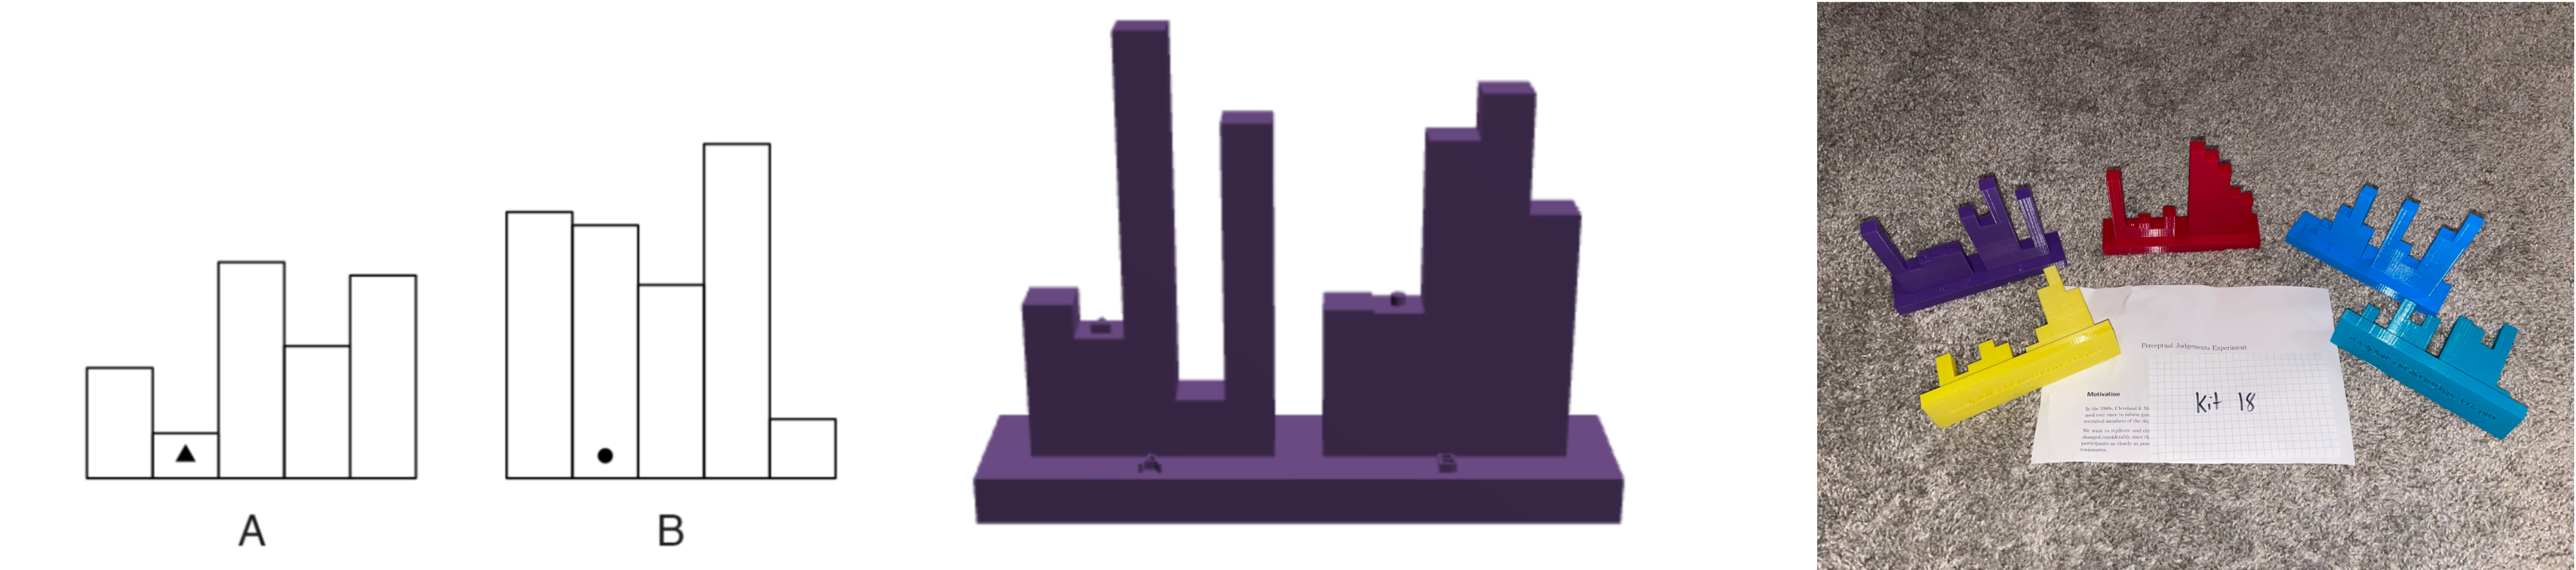
\includegraphics[width=3.125in,height=\textheight]{plot-types.png}

The ggplot2 package was utilized to create the 2D bar charts.
The scale axis was removed, leaving only the bars and a bar grouping identifier.
The bars used for comparisons had the identifying mark at a height of 5 out of 100 for the 2D plots, and the 3D plots had the identifying marks on top of the bars.

For the 3D printed charts, the identifying marks were raised by a marginal amount so that they can be immediately identified after printing.
Other non-data related elements were also raised for the same reason.
A negative-space engraving on the bottom of the 3D printed graph uniquely identifies each graph.
Graphs were printed with colored filament that correspond to a color coordinated ratio comparison.
The ratios were randomly assigned a unique color so that the color does not provide an indication as to what ratio is conveyed.

The digital 3D charts are initially angled to mimic the default 3D bar charts of Microsoft Excel, but the interactivity of Shiny will allow users to adjust the viewing angle.
For a homogeneous appearance of data elements, the digital 3D graphs are colored versions of the STL files used to create the 3D printed graphs.
The colors of the 3D graphs were linked to the ratio of the comparison values so that it was easier to sort the graphs.
Each ratio was randomly assigned a color and any information linking the color to ratio was hidden from participants.

\hypertarget{study-design}{%
\subsection{Study Design}\label{study-design}}

In the spirit of replicating Cleveland and McGill's study, members of our Statistics department and their spouses/partners were asked to participate in our study.
Participants were provided a single kit that has five of seven unique ratio comparisons where each ratio is applied to all three chart types.
There are 21 kits in total so that each combination of ratios is accounted for.
Each graph is randomly assigned either an adjacent or separated comparison.

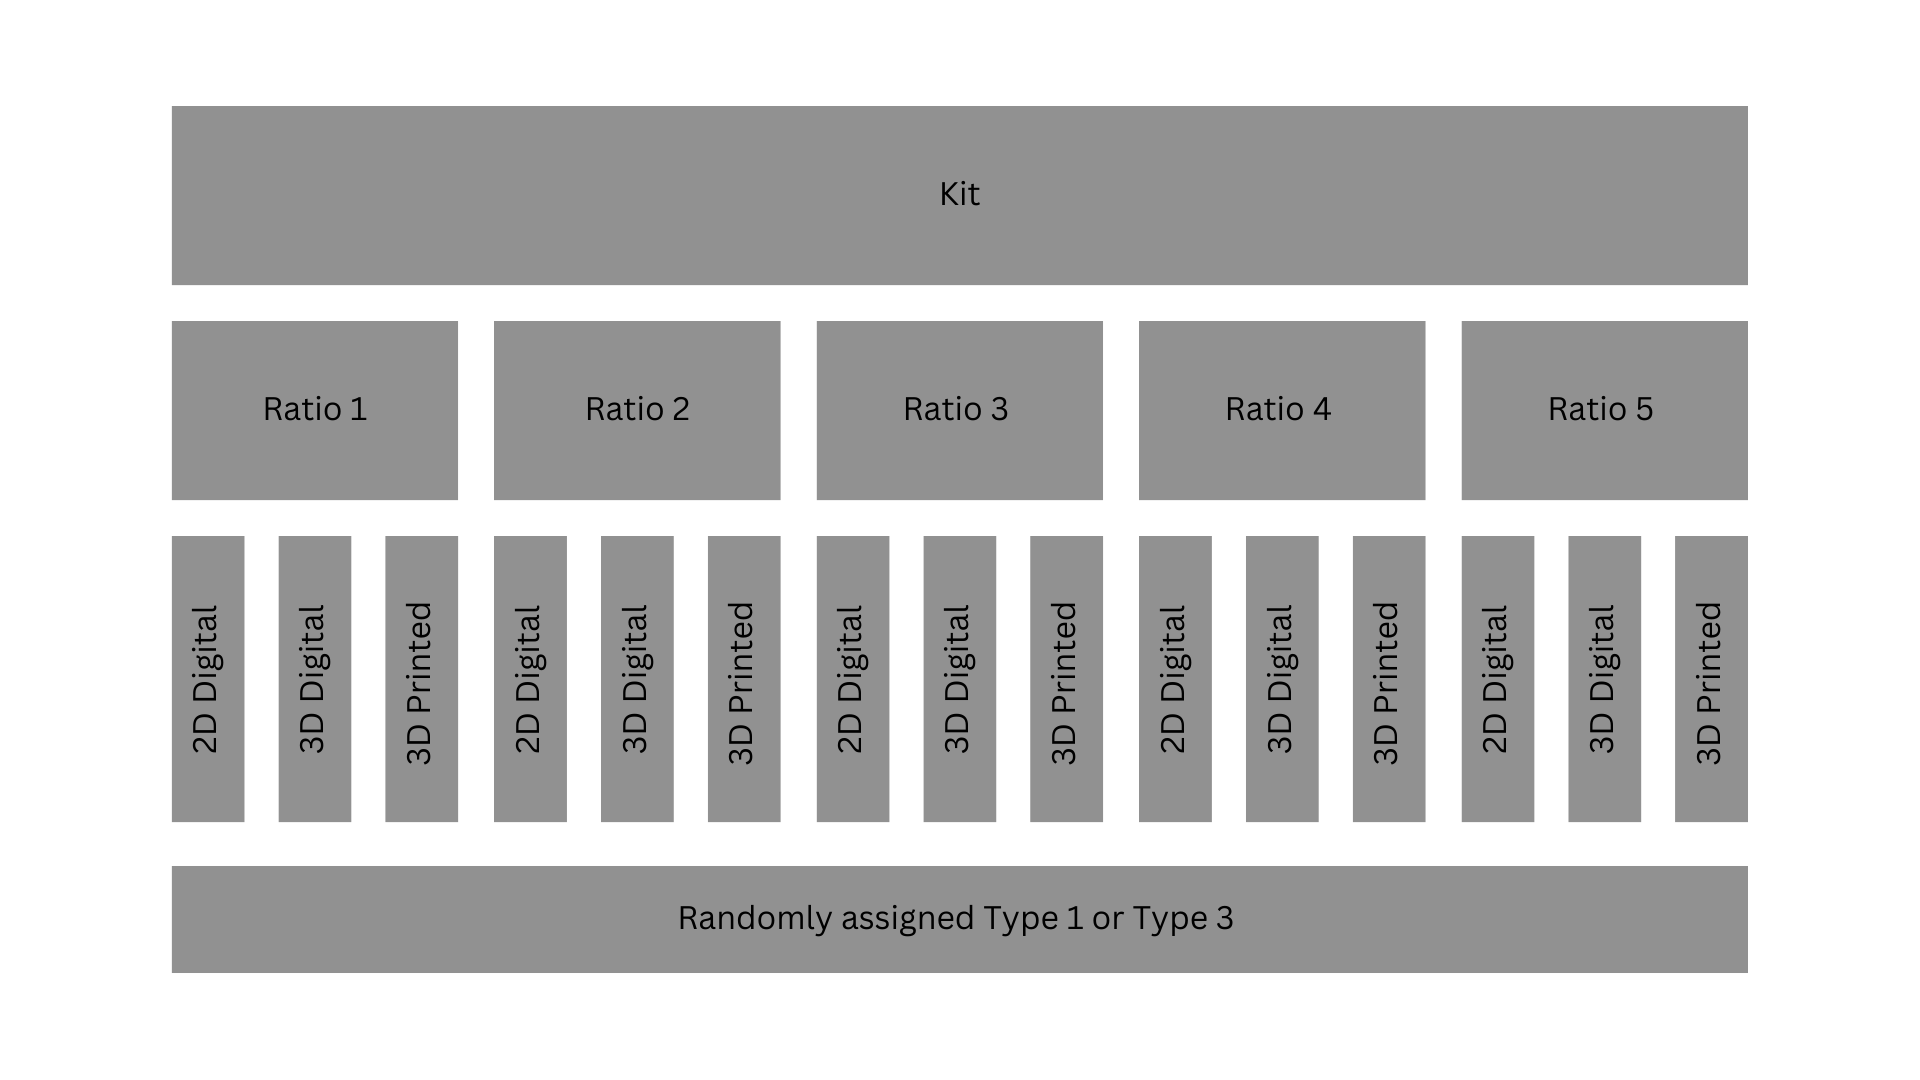
\includegraphics{study-design.png}

A Shiny application on a single computer is used to administer the graphs and questions to participants in a random order.
Participants are provided a few sample graphs before receiving the graphs in their randomly assigned kit.
Prior to answering questions, participants are instructed to make quick judgements for each graph and not to estimate the ratios using physical objects, such as their fingers or pencils.
For the 3D printed graphs, the Shiny application directs participants to a colored graph in a bag and to verify the identifier on the bottom of the graph.

Each graph has two accompanying questions asking which bar is smaller and what the ratio of the smaller bar is to the larger bar.
Participants are presented radio buttons to identify the smaller bar and a slider to input a ratio judgement.

Participant responses are measured by log error of the distance between the true ratio and the participant ratio judgement.

\hypertarget{results}{%
\section{Results}\label{results}}

The data was analyzed with the same log error that was used by Cleveland and McGill. This is presented as the following linear mixed effects model.

\[y_{ijklm}=\mu+S_i+R_j+G(R)_{(k)j}+T_l+\epsilon_{ijklm}\]

\noindent where

\begin{itemize}
\item
  \(y_{ijklm}=\log_2(|\text{Judged Percent} - \text{True Percent}|+1/8)\)
\item
  \(S_i\sim N(0,\sigma^2_S)\) is the effect of the \(i^{th}\) subject
\item
  \(R_j\) is the effect of the \(j^{th}\) ratio
\item
  \(G(R)_{(k)j}\) is the effect of the \(k^{th}\) graph type nested in the \(j^{th}\) ratio
\item
  \(T_l\) is the effect of the \(l^{th}\) comparison type
\item
  \(\epsilon_{ijklm}\sim N(0,\sigma^2_\epsilon)\) is the random error
\end{itemize}

A total of 39 subjects participated in the study.
All responses that incorrectly identified the smaller bar were removed.
No differences were detected for the true ratio of bars (p-value = .689), whether the bars were adjacent or separated (p-value = .220), or for the plot nested within the true ratio (p-value = .837).

\hypertarget{discussion-and-future-work}{%
\section{Discussion and Future Work}\label{discussion-and-future-work}}

Previous work in 3D graphics would suggest that the errors for the 3D graphs would be larger than the errors for the 2D graphs. The results from our study with 39 participants does not reach the same conclusion, but this could possibly be attributed to the small sample size or that the 3D graphs were not from designed like those found in Microsoft Excel. Incorporating a larger sample size and typical 3D graphs will help to replicate previous work and test if the projections of 3D graphs is the limiting factor in the ability to accurately draw comparisons.

The goal of this study was to verify that previous research into graphics is upheld under a new set of circumstances. It started with a question, followed by research into prior work, and then by designing and conducting a study. This general framework of research is useful to all fields of study and is taught in most introductory statistics courses. The next step of this study is to collect more data while simultaneously providing students the opportunity to learn about the research process from both the perspectives of an experiment participant and the views of the researchers. At University of Nebraska-Lincoln, students taking introductory statistics will have the opportunity to participate in the experiment while also completing pre/post experiment surveys and reflections on a two-page abstract and a presentation of results.

Future iterations of this study will include ``traditional'' 3D graphs created by Microsoft Excel and provide the option for online participants to remove the 3D printed graphs from the graphs in their kit. At the final conclusion of the study, we will release a repository to encourage replication and sharing of experimental results.

\newpage

\hypertarget{notes}{%
\section{NOTES}\label{notes}}

\begin{itemize}
\item
  Need to update image
\item
  Work on lit review
\item
  Everything on next pages are kept only for reference. Remove these when draft is ready
\end{itemize}

\newpage

\hypertarget{tables}{%
\section{Tables}\label{tables}}

We recommend \LaTeX~package \texttt{booktabs} for professional
looking tables. Its toprule and bottomrule are thicker than midrule.

A professional table contains no vertical lines.

\hypertarget{figures}{%
\section{Figures}\label{figures}}

Vector graphics do not lose clarity when being scaled. Make your
figure in pdf format when you first generate it and keep in mind its
sizes in the article to avoid over-scaling. Do not simply convert a
jpeg or png image to a pdf.

\hypertarget{code}{%
\section{Code}\label{code}}

The document class \texttt{jds} provides several commands to decorate

\begin{itemize}
\item inline code, such as \code{print("Hello world!")};
\item programming language, such as \proglang{R}, \proglang{Python}, and
  \proglang{C++};
\item software package, such as \pkg{stats}, \pkg{utils}.
\end{itemize}

\begin{Shaded}
\begin{Highlighting}[]
\DocumentationTok{\#\# Dobson (1990) Page 93: Randomized Controlled Trial :}
\NormalTok{counts }\OtherTok{\textless{}{-}} \FunctionTok{c}\NormalTok{(}\DecValTok{18}\NormalTok{, }\DecValTok{17}\NormalTok{, }\DecValTok{15}\NormalTok{, }\DecValTok{20}\NormalTok{, }\DecValTok{10}\NormalTok{, }\DecValTok{20}\NormalTok{, }\DecValTok{25}\NormalTok{, }\DecValTok{13}\NormalTok{, }\DecValTok{12}\NormalTok{)}
\NormalTok{outcome }\OtherTok{\textless{}{-}} \FunctionTok{gl}\NormalTok{(}\DecValTok{3}\NormalTok{, }\DecValTok{1}\NormalTok{, }\DecValTok{9}\NormalTok{)}
\NormalTok{treatment }\OtherTok{\textless{}{-}} \FunctionTok{gl}\NormalTok{(}\DecValTok{3}\NormalTok{, }\DecValTok{3}\NormalTok{)}
\NormalTok{glm.D93 }\OtherTok{\textless{}{-}} \FunctionTok{glm}\NormalTok{(counts }\SpecialCharTok{\textasciitilde{}}\NormalTok{ outcome }\SpecialCharTok{+}\NormalTok{ treatment, }\AttributeTok{family =} \FunctionTok{poisson}\NormalTok{())}
\FunctionTok{summary}\NormalTok{(glm.D93)}
\end{Highlighting}
\end{Shaded}

\begin{verbatim}

Call:
glm(formula = counts ~ outcome + treatment, family = poisson())

Deviance Residuals: 
       1         2         3         4         5         6         7         8  
-0.67125   0.96272  -0.16965  -0.21999  -0.95552   1.04939   0.84715  -0.09167  
       9  
-0.96656  

Coefficients:
              Estimate Std. Error z value Pr(>|z|)    
(Intercept)  3.045e+00  1.709e-01  17.815   <2e-16 ***
outcome2    -4.543e-01  2.022e-01  -2.247   0.0246 *  
outcome3    -2.930e-01  1.927e-01  -1.520   0.1285    
treatment2  -3.242e-16  2.000e-01   0.000   1.0000    
treatment3  -2.148e-16  2.000e-01   0.000   1.0000    
---
Signif. codes:  0 '***' 0.001 '**' 0.01 '*' 0.05 '.' 0.1 ' ' 1

(Dispersion parameter for poisson family taken to be 1)

    Null deviance: 10.5814  on 8  degrees of freedom
Residual deviance:  5.1291  on 4  degrees of freedom
AIC: 56.761

Number of Fisher Scoring iterations: 4
\end{verbatim}

\hypertarget{guide-for-authors}{%
\section{Guide for Authors}\label{guide-for-authors}}

The following requirements must be followed as closely as possible. A
technically acceptable manuscript that fails to follow these requirements may be
returned for retyping, leading to delay in publication.We only accept
submissions in PDF format. The Latex file must be provided after the manuscript
is accepted.

\hypertarget{submission-of-papers}{%
\subsection{Submission of Papers}\label{submission-of-papers}}

Submission of a manuscript must be the original work of the author(s) and have
not been published elsewhere or under consideration for another publication, or
a substantially similar form in any language.

Authors are encouraged to recommend three to five individuals (including their
research fields, e-mail, phone numbers and addresses) who are qualified to serve
as referees for their paper.

\hypertarget{citing-references}{%
\section{Citing References}\label{citing-references}}

The citations are in the author-year format with the
\texttt{jds} bibstyle.

Citations can be in either text or parenthesis format style with
\texttt{$\backslash$citet} or \texttt{$\backslash$citep},
respectively. For example, \citet{KoenkerBassett1978} is a seminal
work on quantile regression; The Laplace distribution has applications
in many fields \citep{Kotz2001}.

\bibliography{JDS2023.bib}
\bibliographystyle{jds}


\end{document}
